\documentclass[fleqn]{beamer}

\usetheme{Rochester}
\setbeamertemplate{navigation symbols}{}

\usepackage[style=alphabetic,maxalphanames=6]{biblatex}
\bibliography{quantitative}

\usepackage{amsmath}
\usepackage{amssymb}
\usepackage{cmll}
\usepackage{ebproof}
\usepackage{ebproof-rules}
\usepackage{mathpartir}
\usepackage{mathrsfs}
\usepackage{mathtools}
%\usepackage{natbib}
\usepackage{turnstile}

\usepackage{tikz}
\usetikzlibrary{tikzmark,fit}

\definecolor{use}{HTML}{008000}
\newcommand\gr[1]{{\color{use}#1}}
\newcommand\grctx[1]{\gr{\mathcal{#1}}}
\newcommand\grP{\grctx P}
\newcommand\grQ{\grctx Q}
\newcommand\grR{\grctx R}
\newcommand\grPprime{\grP\gr'}
\newcommand\grQprime{\grQ\gr'}
\newcommand\name{\ensuremath{\lambda\grR}}
\newcommand\grctxsub[2]{\grctx{#1}_{\gr{#2}}}
\newcommand\grPe{\grctxsub P e}
\newcommand\grPf{\grctxsub P f}
\newcommand\grQe{\grctxsub Q e}
\newcommand\grQf{\grctxsub Q f}
\newcommand\sem[1]{\left\llbracket{#1}\right\rrbracket}
\newcommand\size[1]{\left\lvert{#1}\right\rvert}
\newcommand\ps{\mathit{ps}}
\newcommand\qs{\mathit{qs}}
\newcommand\rs{\mathit{rs}}
\newcommand\dotto{\mathrel{\dot\to}}
\newcommand\dottimes{\mathbin{\dot\times}}
\newcommand\wand{\mathrel{\mathord{-}\hspace{-0.75ex}*}}
\newcommand\sep{\mathbin{*}}
\newcommand\env[1]{(#1\mathrm{-Env})}
\newcommand\thinningN{\mathrm{Thinning}}
\newcommand\thinning[2]{\thinningN~#1~#2}
\newcommand\V{\mathcal V}
\newcommand\C{\mathcal C}
\newcommand\sqin{\mathrel{\mathrlap{\sqsubset}{\mathord{-}}}}
\newcommand\sqni{\mathrel{\mathrlap{\sqsupset}{\mathord{-}}}}
\newcommand\subres{=}
\newcommand\Ann{\mathscr R}

\renewcommand\land{~\wedge~}
\renewcommand\lor{~\vee~}

\DeclareMathOperator\obj{Obj}
\let\hom\relax
\DeclareMathOperator\hom{Hom}
\DeclareMathOperator\id{id}
\DeclareMathOperator\sub{Sub}


\newcommand\Set{\mathrm{Set}}

\title{A Framework for Substructural Type Systems}
\author{James Wood\inst{1} \and Robert Atkey\inst{1}}
\institute{\inst{1}University of Strathclyde}
\date{ESOP, \today}

\ebproofnewstyle{small}{%
  separation=1em,%
  rule margin=.5ex,%
  template=\footnotesize$\inserttext$%
}
\ebproofnewstyle{equiv}{%
  rule style=double%
}

\begin{document}

\frame{\titlepage}

\begin{frame}{Mechanisation of type systems}
  \begin{itemize}
    \item Boring syntactic operations and lemmas
    \item Learn how to do syntax well~\cite{AR99,McBride05,bhkm12}.
    \item Substructural systems are even harder!
  \end{itemize}
\end{frame}

\begin{frame}{Frameworks for type theories}
  \begin{itemize}
    \item A framework for substructural type systems in a general-purpose proof assistant (Agda)
    \item Prior work: simple types~\cite{AACMM21}
      \begin{itemize}
        \item Renaming and substitution for \emph{all} syntaxes
        \item Renaming/substitution fusion laws
        \item Scope checking, type checking
        \item Printing, optimisation passes, NbE
      \end{itemize}
    \item This work: similar for \emph{linear} and \emph{modal} type systems.
      \begin{itemize}
        \item DILL~\cite{Barber1996}, modal S4~\cite{judgmental}, graded~\cite{Granule18}
        \item Semiring-annotated usage-aware calculi
      \end{itemize}
  \end{itemize}
\end{frame}

%\begin{frame}{Prior work: structural case}
%  \begin{block}{Easy simultaneous substitution}
%    \vspace{0.8em}
%    \begin{columns}
%      \begin{column}{.4\linewidth}
%        \[
%          \begin{prooftree}[small]
%            \hypo{\tikzmarknode{app-func-l}{\Delta} \vdash M : A \to B}
%            \hypo{\tikzmarknode{app-arg-l}{\Delta} \vdash N : A}
%            \infer2{\tikzmarknode{app-conc-l}{\Delta} \vdash M\,N : B}
%          \end{prooftree}
%        \]
%      \end{column}
%      \begin{column}{.6\linewidth}
%        \[
%          \begin{prooftree}[small]
%            \hypo{\tikzmarknode{app-func-r}{\Gamma} \vdash M[\sigma] : A \to B}
%            \hypo{\tikzmarknode{app-arg-r}{\Gamma} \vdash N[\sigma] : A}
%            \infer2{\tikzmarknode{app-conc-r}{\Gamma} \vdash (M\,N)[\sigma] : B}
%          \end{prooftree}
%        \]
%      \end{column}
%    \end{columns}
%    \begin{tikzpicture}[overlay, remember picture, shorten >= 2pt, shorten <= 2pt, font=\footnotesize]
%      \draw[<-] (app-conc-l.south) to[bend right=15] node[below]{$\sigma : \Gamma \Rightarrow \Delta$} (app-conc-r.south);
%      \draw[<-] (app-func-l.north) to[bend left=15] node[above]{$\sigma$} (app-func-r.north);
%      \draw[<-] (app-arg-l.north) to[bend left=15] node[above]{$\sigma$} (app-arg-r.north);
%    \end{tikzpicture}
%
%    \vspace{2em}
%    $\sigma$ is a term in $\Gamma$ for each variable in $\Delta$.
%  \end{block}
%  \begin{block}{Binding a variable}
%    \vspace{1.3em}
%    \begin{columns}
%      \begin{column}{.5\linewidth}
%        \[
%          \begin{prooftree}[small]
%            \hypo{\tikzmarknode{lam-body-l}{\Delta, x : A} \vdash M : B}
%            \infer1{\tikzmarknode{lam-conc-l}{\Delta} \vdash \lambda x.~M : A \to B}
%          \end{prooftree}
%        \]
%      \end{column}
%      \begin{column}{.5\linewidth}
%        \[
%          \begin{prooftree}[small]
%            \hypo{\tikzmarknode{lam-body-r}{\Gamma, x : A} \vdash M[\sigma'] : B}
%            \infer1{\tikzmarknode{lam-conc-r}{\Gamma} \vdash (\lambda x.~M)[\sigma] : A \to B}
%          \end{prooftree}
%        \]
%      \end{column}
%    \end{columns}
%    \begin{tikzpicture}[overlay, remember picture, shorten >= 2pt, shorten <= 2pt, font=\footnotesize]
%      \draw[<-] (lam-conc-l.south) to[bend right=15] node[below]{$\sigma$} (lam-conc-r.south);
%      \draw[<-] (lam-body-l.north) to[bend left=15] node[above]{$\sigma' \coloneqq \sigma, x \mapsto x$} (lam-body-r.north);
%    \end{tikzpicture}
%    \vspace{2em}
%  \end{block}
%\end{frame}

\begin{frame}{Linearity is not simple}
  \begin{itemize}
    \item<1-> Key invariant of \cite{AACMM21}: contexts are only ever\ldots
      \begin{itemize}
        \item added to (binding a variable)
        \item accessed by the variable rule
      \end{itemize}
    \item<1-> Motivates an abbreviated notation for typing rules.
      \begin{mathpar}
        \ebrule{%
          \hypo{\vdash A \to B}
          \hypo{\vdash A}
          \infer2[App]{\vdash B}
        }
        \and
        \ebrule{%
          \hypo{x : A \vdash B}
          \infer1[Lam]{\vdash A \to B}
        }
      \end{mathpar}
    \item<2-> Variables going out of scope:
      \[
        \begin{prooftree}
          \hypo{\Gamma \vdash A}
          \hypo{\Delta \vdash B}
          \infer2{\Gamma, \Delta \vdash A \otimes B}
        \end{prooftree}
      \]
      %\begin{columns}
      %  \begin{column}{.35\linewidth}
      %    \[
      %      \begin{prooftree}
      %        \hypo{\Gamma \vdash A}
      %        \hypo{\Delta \vdash B}
      %        \infer2{\Gamma, \Delta \vdash A \otimes B}
      %      \end{prooftree}
      %    \]
      %  \end{column}
      %  \begin{column}{.65\linewidth}
      %    \begin{tikzpicture}[shorten >= 2pt, shorten <= 2pt, font=\footnotesize]
      %      \node(si) at (-3,0) {$\sigma : \Gamma, \Delta \Rightarrow \Gamma', \Delta'$};
      %      \node(siG) at (0,0.25) {$\Gamma \Rightarrow \Gamma'$};
      %      \node(siD) at (0,-0.25) {$\Delta \Rightarrow \Delta'$};

      %      \draw[->] (si) to node[above]{?} (siG);
      %      \draw[->] (si) to node[below]{?} (siD);
      %    \end{tikzpicture}
      %  \end{column}
      %\end{columns}
    \item<3-> Relying on details of the context:~\cite{wadler91use}
      \[
      \begin{prooftree}
        \hypo{\oc A_1, \ldots, \oc A_n \vdash B}
        \infer1{\oc A_1, \ldots, \oc A_n \vdash \oc B}
      \end{prooftree}
      \]
  \end{itemize}
\end{frame}

\begin{frame}{Semiring usage annotations}
  \begin{itemize}
    \item Enrich the judgemental syntax to account for substructurality.
    \item $\gr{r_1}x_1 : A_1, \ldots, \gr{r_n}x_n : A_n \vdash B$
    \item $\gr{r_1}, \ldots, \gr{r_n} \in \Ann$, where $\Ann$ is a (partially ordered) semiring.
    \item Annotations can appear in types via $\oc\gr r$.
    \item Generalises beyond linearity:~\cite{Granule18,AbelBernardy2020,WA21}
      \begin{itemize}
        \item Linearity: $\Ann = (\{0,1,\omega\}, \ldots)$
        \item S4 modal logic: $\Ann = (\{\text{unused},\text{true},\text{valid}\}, \ldots)$
        \item Monotonicity: $\Ann = (\{{\equiv}, {\uparrow}, {\downarrow}, {\wn}\}, \ldots)$
        \item Exact usage-counting: $\Ann = (\mathbb N, =, +, \times)$
      \end{itemize}
  \end{itemize}
\end{frame}

%\begin{frame}{Bunched connectives, introduction}
%  \begin{itemize}
%    \item Yoneda embedding: for partially ordered monoid $(M, =, +)$,
%      \[Y : M \to [M^{op}, \Set]\]
%    \item Day convolution:
%      \begin{flalign*}
%        &{*} : [M^{op}, \Set] \times [M^{op}, \Set] \to [M^{op}, \Set] \\
%        &\plr{T * U}\,z \coloneqq \{ (t, u) \mid z = x + y, t \in T\,x, u \in U\,y \}
%      \end{flalign*}
%      And its unit:
%      \begin{flalign*}
%        &I^{*} : [M^{op}, \Set] \\
%        &I^{*}\,z \coloneqq \{ {\bullet} \mid z = 0 \}
%      \end{flalign*}
%  \end{itemize}
%\end{frame}
%
%\begin{frame}{Bunched connectives, algebra}
%  \begin{itemize}
%    \item Stating algebraic laws:
%      \begin{flalign*}
%        &{\dotto} : [M^{op}, \Set] \times [M^{op}, \Set] \to [M^{op}, \Set] \\
%        &\plr{T \dotto U}\,x \coloneqq T\,x \to U\,x
%      \end{flalign*}
%      \begin{flalign*}
%        &\forallb{{-}} : [M^{op}, \Set] \to \Set \\
%        &\forallb{T} \coloneqq \Pi x.~T\,x
%      \end{flalign*}
%    \item Example: associativity (true for our definition of $\sep$)
%      \begin{flalign*}
%        &\forallb{(T \sep U) \sep V\ \dot\leftrightarrow\ T \sep (U \sep V)}
%      \end{flalign*}
%    \item All studied by \cite{RPKV20}.
%  \end{itemize}
%\end{frame}
%
%\begin{frame}{Bunched connectives, algebraic proofs}
%  Interchange: $\forallb{(T \sep U) \sep (V \sep W) \dotto (T \sep V) \sep (U \sep W)}$
%  \begin{align*}
%    (T \sep U) \sep (V \sep W)
%    &\stackrel\alpha\longrightarrow T \sep (U \sep (V \sep W)) \\
%    &\stackrel{1 \sep \alpha^{-1}}\longrightarrow T \sep ((U \sep V) \sep W) \\
%    &\stackrel{1 \sep (\sigma \sep 1)}\longrightarrow T \sep ((V \sep U) \sep W) \\
%    &\stackrel{1 \sep \alpha}\longrightarrow T \sep (V \sep (U \sep W)) \\
%    &\stackrel{\alpha^{-1}}\longrightarrow (T \sep V) \sep (U \sep W)
%  \end{align*}
%\end{frame}

\begin{frame}{Tensor-introduction}
  \begin{mathpar}
    \ebrule{%
      \hypo{\gr{r_1}x_1 : A_1, \ldots, \gr{r_n}x_n : A_n \vdash B}
      \hypo{\gr{s_1}x_1 : A_1, \ldots, \gr{s_n}x_n : A_n \vdash C}
      \infer2{(\gr{r_1}+\gr{s_1})x_1 : A_1, \ldots, (\gr{r_n}+\gr{s_n})x_n : A_n \vdash B \otimes C}
    }
  \end{mathpar}
  \pause
  \begin{columns}
    \begin{column}{.33\linewidth}
      \begin{mathpar}
        \ebrule{%
          \hypo{\grP\gamma \vdash B}
          \hypo{\grQ\gamma \vdash C}
          \infer2{(\grP + \grQ)\gamma \vdash B \otimes C}
        }
      \end{mathpar}
    \end{column}
    \pause
    \begin{column}{.67\linewidth}
      \begin{mathpar}
        \ebrule{%
          \hypo{\grP\gamma \vdash B}
          \hypo{\grQ\gamma \vdash C}
          \hypo{\grR = \grP + \grQ}
          \infer3{\grR\gamma \vdash B \otimes C}
        }
      \end{mathpar}
    \end{column}
  \end{columns}
  \pause\vspace{1em}
  \begin{mathpar}
    \ebrule[comb]{%
      \hypo{\vdash B}
      \hypo{*}
      \hypo{\vdash C}
      \infer3{\vdash B \otimes C}
    }
  \end{mathpar}
\end{frame}

\begin{frame}{With-introduction}
  \begin{mathpar}
    \ebrule{%
      \hypo{\gr{r_1}x_1 : A_1, \ldots, \gr{r_n}x_n : A_n \vdash B}
      \hypo{\gr{r_1}x_1 : A_1, \ldots, \gr{r_n}x_n : A_n \vdash C}
      \infer2{\gr{r_1}x_1 : A_1, \ldots, \gr{r_n}x_n : A_n \vdash B \with C}
    }
  \end{mathpar}
  \pause\vspace{1em}
    \begin{mathpar}
      \ebrule{%
        \hypo{\grR\gamma \vdash B}
        \hypo{\grR\gamma \vdash C}
        \infer2{\grR\gamma \vdash B \with C}
      }
    \end{mathpar}
  \pause\vspace{1em}
  \begin{mathpar}
    \ebrule[comb]{%
      \hypo{\vdash B}
      \hypo{\dottimes}
      \hypo{\vdash C}
      \infer3{\vdash B \with C}
    }
  \end{mathpar}
\end{frame}

\begin{frame}{Bang-introduction}
  \begin{mathpar}
    \ebrule{%
      \hypo{\gr{s_1}x_1 : A_1, \ldots, \gr{s_n}x_n : A_n \vdash B}
      \infer1{\gr{rs_1}x_1 : A_1, \ldots, \gr{rs_n}x_n : A_n \vdash \oc\gr rB}
    }
  \end{mathpar}
  \pause
  \begin{columns}
    \begin{column}{.33\linewidth}
      \begin{mathpar}
        \ebrule{%
          \hypo{\grP\gamma \vdash A}
          \infer1{(\gr r\grP)\gamma \vdash \oc{\gr r} A}
        }
      \end{mathpar}
    \end{column}
    \pause
    \begin{column}{.67\linewidth}
      \begin{mathpar}
        \ebrule{%
          \hypo{\grP\gamma \vdash A}
          \hypo{\grR = \gr r\grP}
          \infer2{\grR\gamma \vdash \oc{\gr r} A}
        }
      \end{mathpar}
    \end{column}
  \end{columns}
  \pause\vspace{1em}
  \begin{mathpar}
    \ebrule[comb]{%
      \hypo{\gr r \cdot ({} \vdash A)}
      \infer1{{} \vdash \oc{\gr r} A}
    }
  \end{mathpar}
\end{frame}

\begin{frame}{Plus-elimination}
    \begin{mathpar}
      \ebrule{%
        \hypo{\grP\gamma \vdash A \oplus B}
        \hypo{\grQ\gamma, \gr1A \vdash C}
        \hypo{\grQ\gamma, \gr1B \vdash C}
        \infer3{(\grP+\grQ)\gamma \vdash C}
      }
    \end{mathpar}
    \vspace{1em}
    \begin{mathpar}
      \ebrule[comb]{%
        \hypo{{} \vdash A \oplus B}
        \hypo{*}
        \hypo{\big(\gr1A \vdash C}
        \hypo{\dottimes}
        \hypo{\gr1B \vdash C\big)}
        \infer5{{} \vdash C}
      }
    \end{mathpar}
\end{frame}

\begin{frame}{Syntax descriptions}
  \begin{align*}
    &\text{Premises}&\mathit{ps}, \mathit{qs}\quad\Coloneqq{}\quad& \Delta \vdash A \\
    &&\quad\mid{}\quad& \dot1 \quad\mid\quad \mathit{ps} \dottimes \mathit{qs} \\
    &&\quad\mid{}\quad& I^* \quad\mid\quad \mathit{ps} * \mathit{qs} \\
    &&\quad\mid{}\quad& \gr r \cdot \mathit{ps}\\
    \\
    &\text{Rule}&\mathit{r} \quad\Coloneqq{}\quad& \mathit{ps} \over {} \vdash A \\
    \\
    &\text{System}&\mathit{s} \quad\coloneqq{}\quad& \Sigma(\mathit{Label} : \Set).~\mathit{Label} \to \mathrm{Rule}
  \end{align*}
  Resembles bunched logic~\cite{RPKV20}.
\end{frame}

\begin{frame}{Variables}
  Basis vector
  \begin{mathpar}
    \ebrule{%
      \infer0{\ldots, \gr0y_k : B_k, \gr1x : A, \gr0y_{k+1} : B_{k+1}, \ldots \vdash x : A}
    }
  \end{mathpar}
  \vspace{1em}
  \begin{mathpar}
    \ebrule{%
      \hypo{\lvert \gamma \rvert \ni i}
      \hypo{\gamma_i = A}
      \infer2{(\langle i \rvert)\gamma \vdash A}
    }
  \end{mathpar}
  \vspace{1em}
  \begin{mathpar}
    \ebrule{%
      \hypo{{} \sqni A}
      \infer1{{} \vdash A}
    }
  \end{mathpar}
  ``System + variables = terms''
\end{frame}

\begin{frame}{Instances}
  We have definitions (in Agda) of:
  \begin{itemize}
    \item Linear/quantitative STLC
    \item Core Granule
    \item Linear/non-linear type theory; $A \Coloneqq \mathop{lin}X \mid \mathop{int}Y$
      \begin{itemize}
        \item Translations to and from L/nL and linear STLC
      \end{itemize}
    \item Classical linear logic via $\mu\tilde\mu$; $A \Coloneqq \mathop{command} \mid \mathop{term}X \mid \mathop{coterm}X$
  \end{itemize}

  Moreover, we have \emph{substitution} for any of these\ldots
\end{frame}

\begin{frame}{Substitution: intuitionistic}
  Let $\Delta = \Delta_1, \ldots, \Delta_n$.
  \vspace{2em}
  \begin{columns}
    \begin{column}{0.33\linewidth}
      \[
        \begin{matrix}
          \Gamma \\
          \Downarrow \\
          \Delta
        \end{matrix}
      \]
    \end{column}
    \begin{column}{0.67\linewidth}
      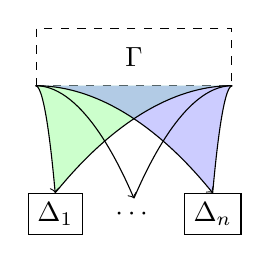
\begin{tikzpicture}[baseline]
        \path
        (-1,1) node (Gtop) {}
        (0,1) node (G) {$\Gamma$}
        (1,1) node (Gbot) {}
        ;
        \node[draw,dashed,fit=(Gtop) (G) (Gbot)] (GG) {};

        \path
        (-1,-1) node[draw] (Dtop) {$\Delta_1$}
        (0,-1) node (D) {$\cdots$}
        (1,-1) node[draw] (Dbot) {$\Delta_n$}
        ;

        \fill[green!20!white,opacity=1] (GG.south west)
        parabola[bend at start] (Dtop.north)
        parabola[bend at end] (GG.south east)
        -- cycle;
        \fill[blue!40!white,opacity=.5] (GG.south west)
        parabola[bend at start] (Dbot.north)
        parabola[bend at end] (GG.south east)
        -- cycle;

        \draw[->] (GG.south west) parabola[bend at start] (Dtop.north);
        \draw (GG.south east) parabola[bend at start] (Dtop.north);
        \draw[->] (GG.south west) parabola[bend at start] (D.north);
        \draw (GG.south east) parabola[bend at start] (D.north);
        \draw[->] (GG.south west) parabola[bend at start] (Dbot.north);
        \draw (GG.south east) parabola[bend at start] (Dbot.north);
      \end{tikzpicture}
    \end{column}
  \end{columns}
  \[
    \forall A.~\Delta \ni A \to \Gamma \vdash A
  \]
\end{frame}

\begin{frame}{Substitution: linear}
  Let $\Gamma = \grP\gamma$ and $\Delta = \grQ_1\delta_1, \ldots, \grQ_n\delta_n$.
  \vspace{1em}
  \begin{columns}
    \begin{column}{0.67\linewidth}
      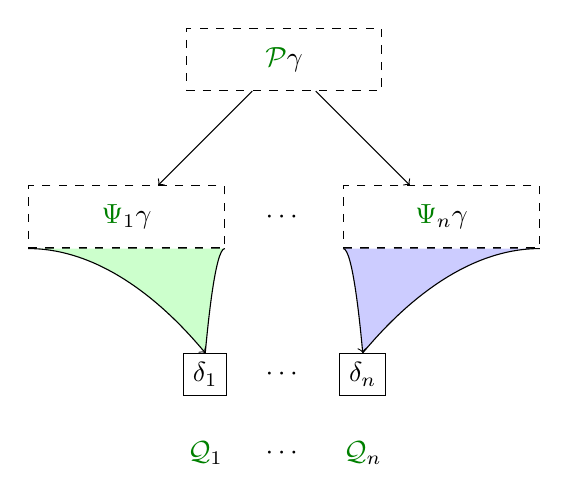
\begin{tikzpicture}[baseline]
        \path
        (-1,1) node (Gtop) {}
        (0,1) node (G) {$\grP\gamma$}
        (1,1) node (Gbot) {}
        ;
        \node[draw,dashed,fit=(Gtop) (G) (Gbot)] (GG) {};

        \path
        (-3,-1) node (G1top) {}
        (-2,-1) node (G1) {$\gr\Psi_1\gamma$}
        (-1,-1) node (G1bot) {}
        ;
        \node[draw,dashed,fit=(G1top) (G1) (G1bot)] (GG1) {};
        \draw[->] (GG) -- (GG1);

        \path (0,-1) node {$\cdots$};

        \path
        (1,-1) node (Gntop) {}
        (2,-1) node (Gn) {$\gr\Psi_n\gamma$}
        (3,-1) node (Gnbot) {}
        ;
        \node[draw,dashed,fit=(Gntop) (Gn) (Gnbot)] (GGn) {};
        \draw[->] (GG) -- (GGn);

        \path
        (-1,-3) node[draw] (Dtop) {$\delta_1$}
        (0,-3) node (D) {$\cdots$}
        (1,-3) node[draw] (Dbot) {$\delta_n$}
        ;

        \path
        (-1,-4) node (Qtop) {$\grQ_1$}
        (0,-4) node (Q) {$\cdots$}
        (1,-4) node (Qtop) {$\grQ_n$}
        ;

        \fill[green!20!white] (GG1.south west)
        parabola[bend at start] (Dtop.north)
        parabola[bend at end] (GG1.south east)
        -- cycle;
        \draw[->] (GG1.south west) parabola[bend at start] (Dtop.north);
        \draw (GG1.south east) parabola[bend at start] (Dtop.north);

        \fill[blue!20!white] (GGn.south west)
        parabola[bend at start] (Dbot.north)
        parabola[bend at end] (GGn.south east)
        -- cycle;
        \draw[->] (GGn.south west) parabola[bend at start] (Dbot.north);
        \draw (GGn.south east) parabola[bend at start] (Dbot.north);
      \end{tikzpicture}
    \end{column}
    \begin{column}{0.33\linewidth}
      \uncover<1->{%
        \[
          \grP = \sum_i{\grQ_i\gr\Psi_i}
        \]
      }
      \uncover<2->{%
        i.e.
        \[
          \grP = \grQ\gr\Psi
        \]
      }
    \end{column}
  \end{columns}
\end{frame}

\begin{frame}{Substitution}
  \begin{itemize}
    \item A substitution is based around a \emph{linear} transformation.
    \item Using the linearity, substitutions commute with addition and scaling.
    \item We can deal with bunched connectives, and also variable-binding, so substitution works.
  \end{itemize}
  \pause
  Substitution generalises to \emph{traversal} over terms\ldots
  \begin{itemize}
    \item Replace $\vdash$ by $\sqni$ to get \emph{simultaneous renaming}.
    \item Replace $\vdash$ by semantic morphisms to get a denotational semantics.
  \end{itemize}
\end{frame}

%\begin{frame}{Substitution: properties}
%  Build substitutions inductively:
%  \begin{mathpar}
%    \ebrule[comb,equiv]{%
%      \hypo{I^*}
%      \infer1{{} \Rightarrow {\cdot}}
%    }
%    \and
%    \ebrule[comb,equiv]{%
%      \hypo{{} \Rightarrow \Delta_l}
%      \hypo{\sep}
%      \hypo{{} \Rightarrow \Delta_r}
%      \infer3{{} \Rightarrow \Delta_l, \Delta_r}
%    }
%    \and
%    \ebrule[comb,equiv]{%
%      \hypo{\gr r\cdot\plr{{} \vdash A}}
%      \infer1{{} \Rightarrow \gr rA}
%    }
%  \end{mathpar}
%
%  \pause
%
%  Pass substitutions over connectives:
%  \begin{mathpar}
%    \ebrule[equiv]{%
%      \hypo{\Gamma \Rightarrow \Delta}
%      \hypo{\Delta = \vec 0}
%      \infer2{\Gamma = \vec 0}
%    }
%    \and
%    \ebrule[equiv]{%
%      \hypo{\Gamma \Rightarrow \Delta}
%      \hypo{\Delta = \Delta_l + \Delta_r}
%      \infer2{\Gamma = \Gamma_l + \Gamma_r
%        \hspace{1.5em} \Gamma_l \Rightarrow \Delta_l
%        \hspace{1.5em} \Gamma_r \Rightarrow \Delta_r}
%    }
%    \and
%    \ebrule[equiv]{%
%      \hypo{\Gamma \Rightarrow \Delta}
%      \hypo{\Delta = \gr r\Delta'}
%      \infer2{\Gamma = \gr r\Gamma'
%        \hspace{1.5em} \Gamma' \Rightarrow \Delta'}
%    }
%  \end{mathpar}
%
%  \pause
%
%  Replace $\vdash$ by $\sqni$ to get \emph{simultaneous renaming}.
%\end{frame}

%\begin{frame}{Substitution: lookup}
%  \begin{itemize}
%    \item Intuitionistically: $\forall A.~\Delta \ni A \to \Gamma \vdash A$.
%    \item Linearly, it is quite rare to have $\Delta \sqni A$.
%  \end{itemize}
%\end{frame}

\begin{frame}{Results}
  \begin{itemize}
    \item Back in the room: AACMM-style semantic traversal follows.
      \begin{itemize}
        \item Refine between $\dottimes$ and $*$, and $\dotto$ and $\wand$.
      \end{itemize}
    \item Renaming and substitution for \emph{all} syntaxes we can describe
      \begin{itemize}
        \item E.g: DILL, S4 modal logic, core Granule, L/nL, classical $\mu\tilde\mu$
        \item We add a $\Box$ connective for \emph{duplicable} premises, e.g recursion.
      \end{itemize}
    \item A generic usage elaborator for \emph{all} these syntaxes
    \item Some tools for denotational semantics
  \end{itemize}
\end{frame}

\begin{frame}{Conclusions}
  \begin{center}
    \url{https://github.com/laMudri/generic-lr/tree/display}
  \end{center}
  \begin{itemize}
    \item Lesson: we can adapt an intuitionistic framework when we understand\ldots
      \begin{itemize}
        \item the algebra of contexts, and
        \item what it means to \emph{derive} one context from another.
      \end{itemize}
    \item Future work:
      \begin{itemize}
        \item Explore expressibility of typing rules.
        \item Try other substructural disciplines $\sim$ other interpretations of the bunched connectives.
        \item Proofs about renaming/substitution (fusion laws)
        \item A generalisation of multicategories
      \end{itemize}
  \end{itemize}
\end{frame}

%\begin{frame}[t, allowframebreaks]{References}
%  \bibliographystyle{alpha}
%  \bibliography{../quantitative}
%\end{frame}

\end{document}
